\documentclass[main.tex]{subfiles}
\begin{document}
\section{Question 4}
Bob works for an auditing agency needs to be able to read all the files in the
system. The system admin has to protect the integrity of the system and should
not allow Bob to modify or delete any file. Write a special SETUID program for
the admin so that he can gave the executable permission of it to Bob. This
program requires Bob to type a file name at the command line and then it will
run /bin/cat to display the specified file. Can Bob compromise the integrity (by
adding/modifying/deleting files) of this system? How?

\lstinputlisting[style=codeStyleC]{listings/4.c}

Bob cannot compromise the system. If he tries to edit any files (by
redirecting), those files are first opened by his shell which does not have root
permissions. /bin/cat does not open any files for writing, and hence the
elevated privileges with which /bin/cat runs cannot be used to modify files if
Bob does not have write permissions to those files in the first place.  This is
why the \texttt{./script | sudo tee FILE} paradigm is used to redirect the
output of a script to a file that is writable by root only. tee opens FILE in
this case and can hence open files for writing with elevated privileges granted
by sudo.

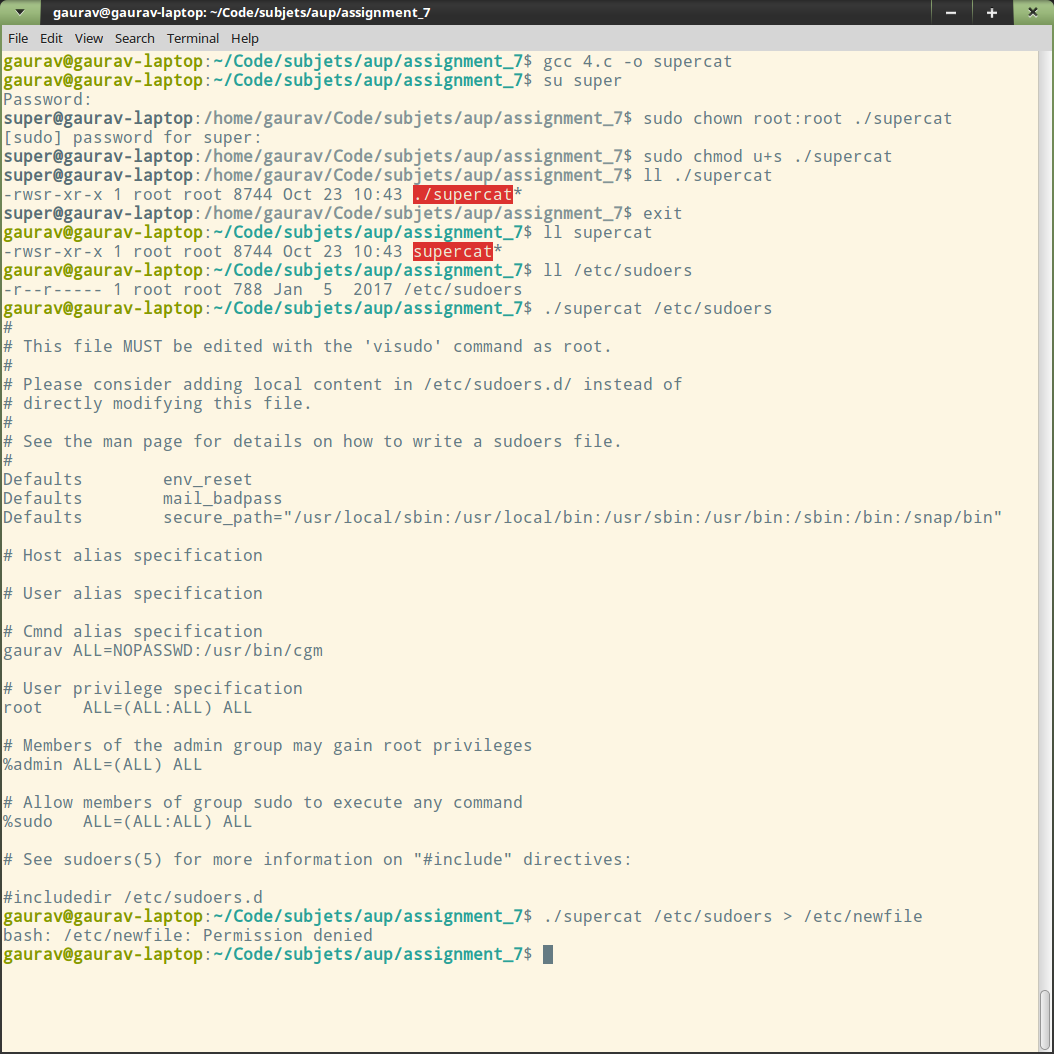
\includegraphics[width=\textwidth]{figures/4_output.png}
\end{document}
